%! Licence = CC BY-NC-SA 4.0

%! Author = gianfluetsch
%! Date = 22. Jan 2022
%! Project = icth_summary

\section{Dauer und Bandbreite von Einzelpulsen}

\subsubsection{Prüfung HS2019}
Ein parabelförmiger Puls s(t) hat folgenden zeitlichen Verlauf:
\begin{center}
    \vspace{-8pt}
    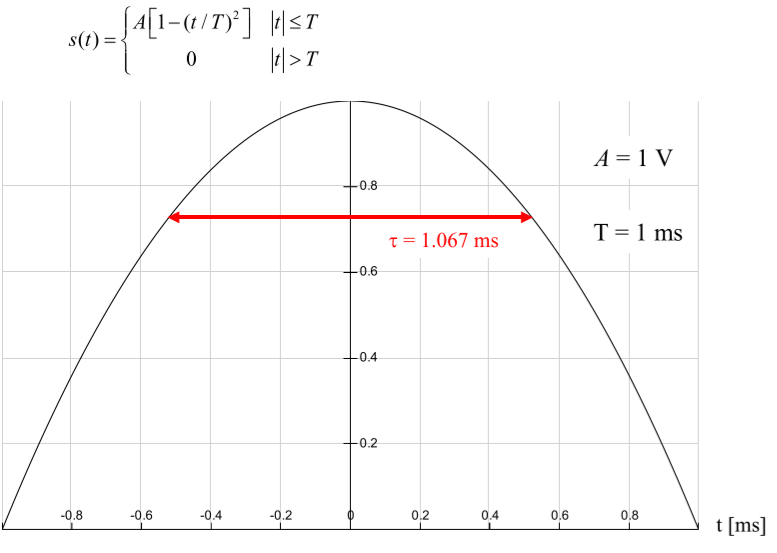
\includegraphics[width=.5\linewidth]{./08-einzelpulse/hs2019}
    \vspace{-8pt}
\end{center}

Das zweiseitige Amplitudendichtespektrum S(f) in [V/Hz] berechnet sich aus dem zeitkontinuierlichen Signal s(t) über die Fouriertransformation zu
\begin{center}
    \vspace{-8pt}
    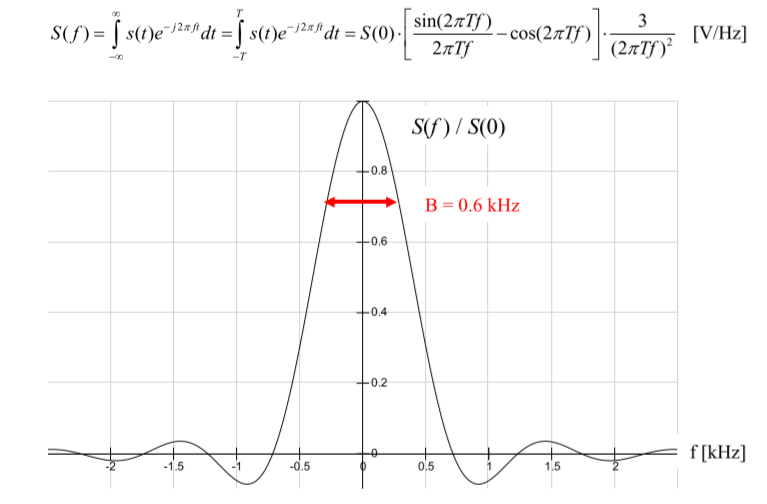
\includegraphics[width=.5\linewidth]{./08-einzelpulse/hs2019_1}
    \vspace{-8pt}
\end{center}

Wie ist das asymptotische Verhalten des Amplitudendichtespektrums S(f) für |f | >> 1?\\
\textit{Quadratische Abnahme mit $1/f^2$}\\

Wie kann S(0), d.h. die Amplitudendichte bei der Frequenz f = 0 Hz aus dem Verlauf des parabelförmigen Pulses s(t) berechnet werden? Benützen Sie als Hilfe die analytische
Lösung des folgenden Integrals:\\
$\int_{-T}^{T} (1-\frac{t^2}{T^2})dt=\frac{4}{3}T$\\

Geben Sie die Formel für S(0), sowie den numerischen Wert in [V/Hz] an\\
Für f=0 gilt: $S(0)=\int_{-\infty}^{\infty}s(t)dt=\int_{-T}^{T}A(1-\frac{t^2}{T^2})dt=\frac{4}{3}AT$\\
\textit{Der numerische Wert ist: S(0) = 4/3 V * 1ms = 1.33 mV/Hz}\\

Die im parabelförmigen Puls s(t) enthaltene Energie kann mit folgender Formel berechnet werden\\
$E=\int_{-\infty}^{\infty}p(t)dt=\int_{-\infty}^{\infty}\frac{s^2(t)}{R}dt=\frac{1}{R}\int_{-T}^{T}s^2(t)dt=\frac{16}{15}\frac{A^2T}{R} [Ws]$\\

Wie gross ist die Energie E in [J] oder [Ws] an einem Widerstand $R = 1 \omega$?\\
$E = 16/15 * 1 V^2 * 1ms / 1 \omega = 16/15 mWs = 1.067 mJ$\\

Wie gross ist die Dauer $\tau$ eines äquivalenten Rechteckpulses $r(t)$ mit Amplitude A und dem gleichen Energieinhalt an $R = 1 \omega$ wie der parabelförmige Puls s(t)? Leiten Sie die Formel for die äquivalente Rechteckdauer $\tau $ als Formel her und bestimmen Sie den numerischen Wert in [s].\\
$A=\frac{A^2\tau}{R}=\frac{16}{15}\frac{A^2T}{R}$\\
$\tau = \frac{16}{15}T$ und damit $\tau =16/15 ms = 1.067ms$\\

Wie gross ist die Bandbreite B eines äquivalenten rechteckförmigen Spektrums mit gleicher Amplitudedichte S(0) und gleichem Energieinhalt an $R = 1 \omega$ wie das Amplitudendichtespektrum S(f) des parabelförmigen Pulses s(t)? Leiten Sie die Formel für die äquivalente Rechteckbandbreite B als Formel her und bestimmen Sie den numerischen Wert in [Hz].\\
$E=\frac{|S(0)|^2B}{R}=\frac{16}{9}\frac{A^2T^2B}{R}=\frac{16}{15}\frac{A^2T}{R}$\\
$B=\frac{3}{5}\frac{1}{T}$ und damit $B=3/5 kHz=0.6kHz$\\

Wie gross ist das Zeit-Bandbreiteprodukt $B_{\tau }$ des parabelförmigen Pulses s(t)?\\
$B_{\tau }=\frac{3}{5}\frac{1}{T}*\frac{16}{15}T=\frac{16}{25}=0.64$

\subsubsection{Prüfung HS2018}
Der sogenannte \textit{Raised-Cosine} Einzelpuls s(t) hat folgenden zeitlichen Verlauf:
\begin{center}
    \vspace{-8pt}
    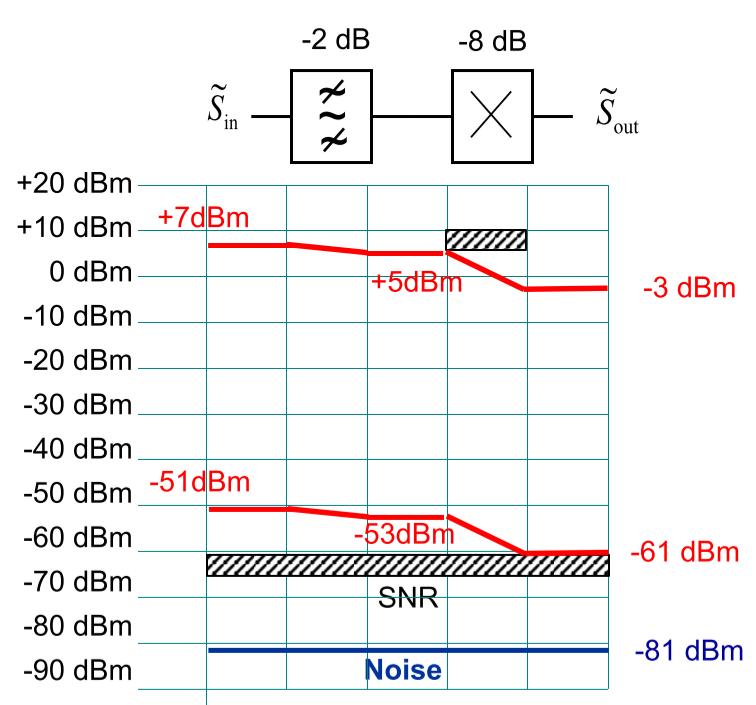
\includegraphics[width=.5\linewidth]{./08-einzelpulse/hs2018}
    \vspace{-8pt}
\end{center}

Das zweiseitige Amplitudendichtespektrum S(f) in [V/Hz] berechnet sich aus dem zeitkontinuierlichen Signal s(t) über die Fouriertransformation zu
\begin{center}
    \vspace{-8pt}
    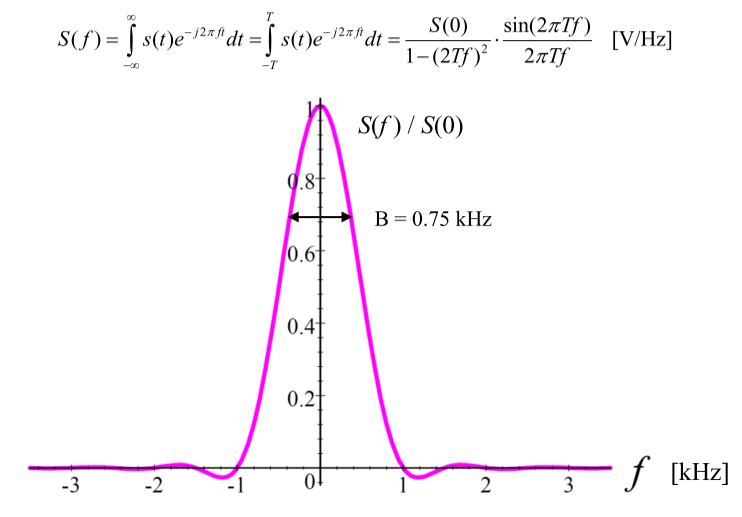
\includegraphics[width=.5\linewidth]{./08-einzelpulse/hs2018_1}
    \vspace{-8pt}
\end{center}

Wie kann S(0), d.h. die Amplitudendichte bei der Frequenz $f=0 Hz$, einfach aus dem Verlauf des Raised-Cosine Pulses s(t) berechnet werden? Geben Sie die Formel für S(0),
sowie den numerischen Wert in [V/Hz] an.\\
Für f = 0 gilt: $S(0)=\int_{-\infty}^{\infty}s(t)dt=\int_{-T}^{T}s(t)dt=AT$\\
\textit{d.h. die Gesamtfläche A/2*2T unter dem Gleichspannungswert, da die Fläche des Cosinus über eine Periode gerade Null ergibt.}\\
\textit{Der nummerische Wert ist:} $S(0)=1V*1ms=1mv/Hz$\\

Die im \textit{Raised-Cosine} Pulse s(t) enthaltene Energie kann mit folgender Formel berechnet werden\\
$E=\int_{-\infty}^{\infty}p(t)dt=\int_{-\infty}^{\infty}\frac{s^2(t)}{R}dt=\frac{1}{R}\int_{-T}^{T}s^2(t)dt=\frac{3}{4}\frac{A^2T}{R}[Ws]$\\

Wie gross ist die Energie E in [J] oder [Ws] an einem Widerstand $R = 1 \omega$?\\
$E = 3/4 * 1 V^2 * 1ms / 1 \omega = 3/4 mWs = 0.75 mJ$\\

Wie gross ist die Dauer $\tau $ eines äquivalenten Rechteckpulses r(t) mit Amplitude A und dem gleichen Energieinhalt an $R = 1 \omega$ wie der Raised-Cosine Puls s(t)? Leiten Sie die Formel for die äquivalente Rechteckdauer $\tau $als Formel her und bestimmen Sie den numerischen Wert in [s].\\
$E=\frac{A^2 \tau }{R}=\frac{3}{4}\frac{A^2T}{R}$\\
$\tau=\frac{3}{4}T$ und damit $\tau=3/4 ms = 0.75ms$\\

Wie gross ist die Bandbreite B eines äquivalenten rechteckförmigen Spektrums mit gleicher Amplitudedichte S(0) und gleichem Energieinhalt an $R = 1 \omega$ wie das Amplitudendichtespektrum S(f) des Raised-Cosine Pulses s(t)? Leiten Sie die Formel für die äquivalente Rechteckbandbreite B als Formel her und bestimmen Sie den numerischen Wert in [Hz].\\
$E=\frac{|S(0)|^2B}{R}=\frac{A^2T^2B}{R}=\frac{3}{4}\frac{A^2T}{R}$\\
$B=\frac{3}{4}\frac{1}{T}$ und damit $\tau = 3/4 kHz = 0.75 kHz$\\

Wie gross ist das Zeit-Bandbreiteprodukt $B_{\tau}$ des Raised-Cosine Pulses s(t)?\\
$B_{\tau}=\frac{3}{4}\frac{1}{T}*\frac{3}{4}T=\frac{9}{16}=0.5625$

\subsubsection{Prüfung HS2017}
Ein dreieckförmiger Einzelpuls s(t) hat folgenden zeitlichen Verlauf:
\begin{center}
    \vspace{-8pt}
    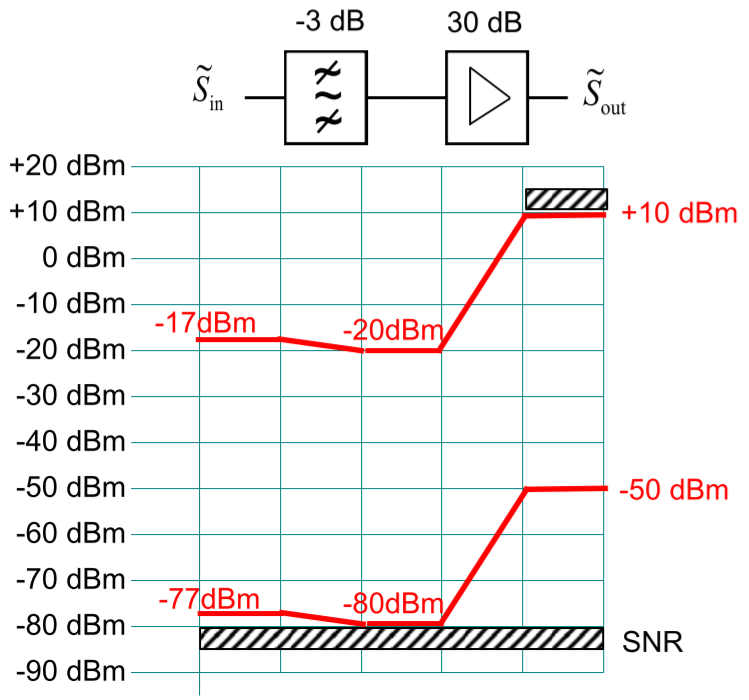
\includegraphics[width=.5\linewidth]{./08-einzelpulse/hs2017}
    \vspace{-8pt}
\end{center}

Das zweiseitige Amplitudendichtespektrum S(f) in [V/Hz] berechnet sich aus dem zeitkontinuierlichen Signal s(t) über die Fouriertransformation zu\\
\begin{center}
    \vspace{-8pt}
    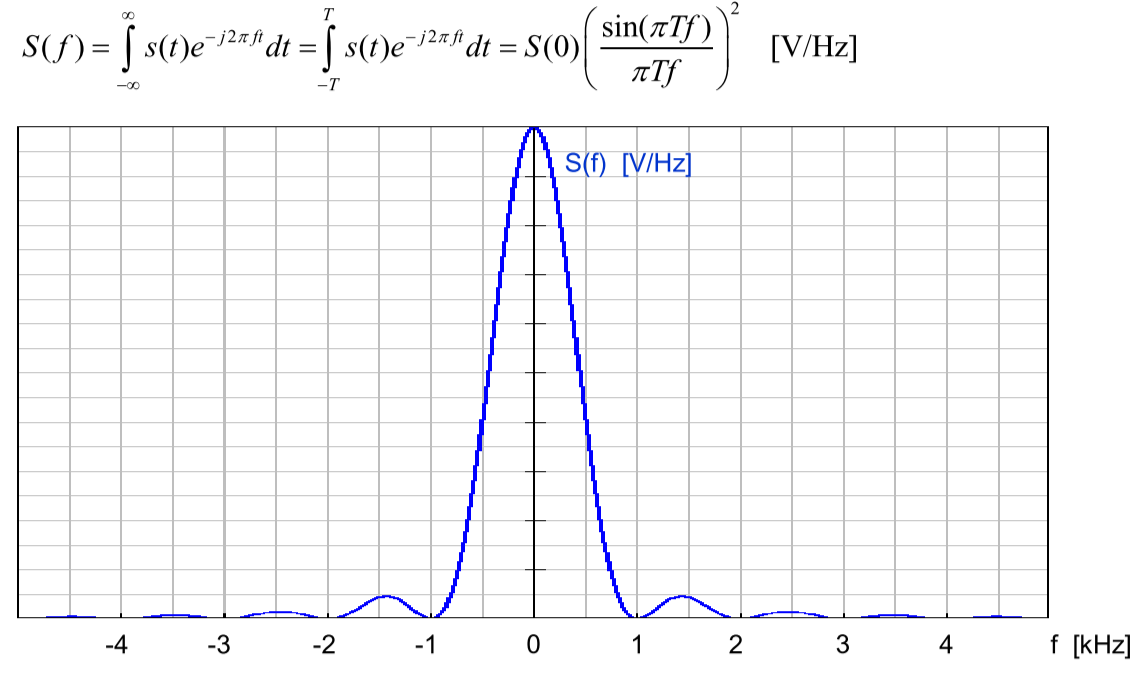
\includegraphics[width=.5\linewidth]{./08-einzelpulse/hs2017_2}
    \vspace{-8pt}
\end{center}

Wie kann S(0), d.h. die Amplitudendichte bei der Frequenz f = 0 Hz, \textbf{einfach} aus dem Verlauf des Dreieckpulses s(t) berechnet werden? Geben Sie die Formel für S(0), sowie
den numerischen Wert in [V/Hz] an.\\
\textit{Für f=0 gilt:} $S(0)=\int_{-\infty}^{\infty}s(t)dt=\int_{-T}^{T}s(t)dt=AT$\\

\textit{d.h. die Gesamtfläche unter der Dreiecksfunktion s(t).}\\
\textit{Der numerische Wert ist:} $S(0)=10V*1ms=10mv/Hz$\\

Die im Dreieckspuls s(t) enthaltene Energie kann mit folgender Formel berechnet werden\\
$E=\int_{-\infty}^{\infty}p(t)dt=\int_{-\infty}^{\infty}\frac{s^2(t)}{R}dt=\frac{1}{R}\int_{-T}^{T}s^2(t)dt=\frac{3}{4}\frac{A^2T}{R}[Ws]$\\

Wie gross ist die Energie E in [J] oder [Ws] an einem Widerstand $R = 50 \omega$?
$E = 2/3 * 100 V^2 * 1ms / 50 \omega = 4/3 mWs = 1.333 mJ$

Wie gross ist die Dauer $\tau$ eines äquivalenten Rechteckpulses r(t) mit Amplitude A und dem gleichen Energieinhalt an $R = 50 \omega$ wie der Dreieckpuls s(t)? Leiten Sie die Formel for die äquivalente Rechteckdauer $\tau$ als Formel her und bestimmen Sie den numerischen
Wert in [s].\\
$E=\frac{A^2 \tau }{R}=\frac{3}{4}\frac{A^2T}{R}$\\
$\tau=\frac{3}{4}T$ und damit $\tau=3/4 ms = 0.75ms$\\

Wie gross ist die Bandbreite B eines äquivalenten rechteckförmigen Spektrums mit gleicher Amplitudedichte S(0) und gleichem Energieinhalt an $R = 50 \omega$ wie das Amplitudendichtespektrum S(f) des Raised-Cosine Pulses s(t)? Leiten Sie die Formel für die äquivalente Rechteckbandbreite B als Formel her und bestimmen Sie den numerischen Wert in [Hz].\\
$E=\frac{|S(0)|^2B}{R}=\frac{A^2T^2B}{R}=\frac{2}{3}\frac{A^2T}{R}$\\
$B=\frac{2}{3}\frac{1}{T}$ und damit $\tau = 2/3 kHz = 0.666 kHz$\\

Wie gross ist das Zeit-Bandbreiteprodukt $B_{\tau}$ des Dreieckpulses s(t)?\\
$B_{\tau}=\frac{2}{3}\frac{1}{T}*\frac{2}{3}T=\frac{4}{9}=0.444$